
In this report, two different types of microphone structures have been analyzed, and the results have been compared with each other and with the reference paper \cite{krishnapriya2014}. \\
The result are quite different from the paper for various reasons

\begin{itemize}
    \item The microphone structure in the paper is not fully defined, so the model used in this work has been built with slight modifications.
    \item The materials of the structure are defined in the paper, but the material properties used in the simulation may differ from those originally used.
    \item The physics modules used to perform the simulations are not specified in the paper.
    \item The mesh used is extremely coarse, this because of the computational cost of the simulation, leading to not accurate results.
\end{itemize}

\noindent
Another aspect to consider is that the structure has been analyzed without considering the air viscosity which introduces a nonlinear relationship between the displacement and the applied pressure. \\
Despite this, the computed results are physically plausible, considering the micromechanical properties of the structure. \\
An improvement to reduce the computational cost of the simulation is to exploit the symmetry of the structure; in fact, we can consider only a quarter of the structure and impose symmetry boundary conditions. \\
This approach could allow us to perform the simulations with a slightly improved mesh quality without increasing their computational cost.

\subsection{Comparison with paper results}

On the reference paper the displacement difference for both structures is larger than the one simulated, but comparing the displacement graph \cite[p.~3, Fig.~3 and Fig.~5]{krishnapriya2014}, with the one simulated (\autoref{fig:3d_displacement_module}) we can observe that the trend of the displacement on the structure is similar even if the values are different. \\
Another consideration that has to be done is that the perforated back structure shows results very close to those reported in the paper, both in terms of maximum displacement and displacement sensitivity. \\
The difference observed for the perforated diaphragm structure may be due to the inclusion of air viscosity effects in the original paper results.

\subsection{Mesh quality impact on results}

Surely the mesh quality introduced an error in the results, for this reason the two structures have been simplified, removing: the backplate, the air, the moving mesh, the parametric simulation and the electrostatic module, to allow the simulation with a better mesh quality and to see how the mesh impacts the final result.

\begin{figure}[h!]
    \centering
    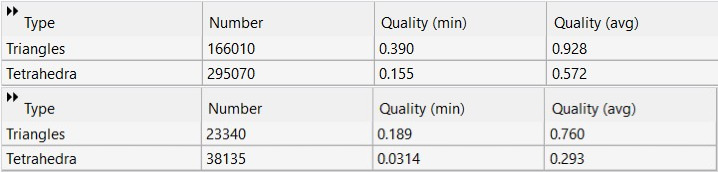
\includegraphics[width=1\linewidth]{img/perf_back_mesh_table.jpg}
    \caption{Number of mesh entities for the perforated back structure: \\
    the upper table is for normal quality mesh, the lower table is for extra-coarse quality mesh}
    \label{fig:perf_back_mesh_table}
\end{figure}

\begin{figure}[h!]
    \centering
    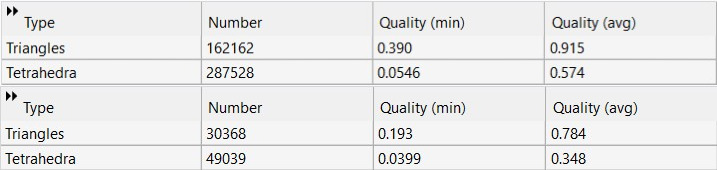
\includegraphics[width=1\linewidth]{img/perf_diap_mesh_table.jpg}
    \caption{Number of mesh entities for the perforated diaphragm structure: \\
    the upper table is for normal quality mesh, the lower table is for extra-coarse quality mesh}
    \label{fig:perf_diap_mesh_table}
\end{figure}

\noindent
The quantity evaluated with this two different type of mesh are the maximum displacement and the maximum stress values.

\begin{figure}[h!]
    \centering
    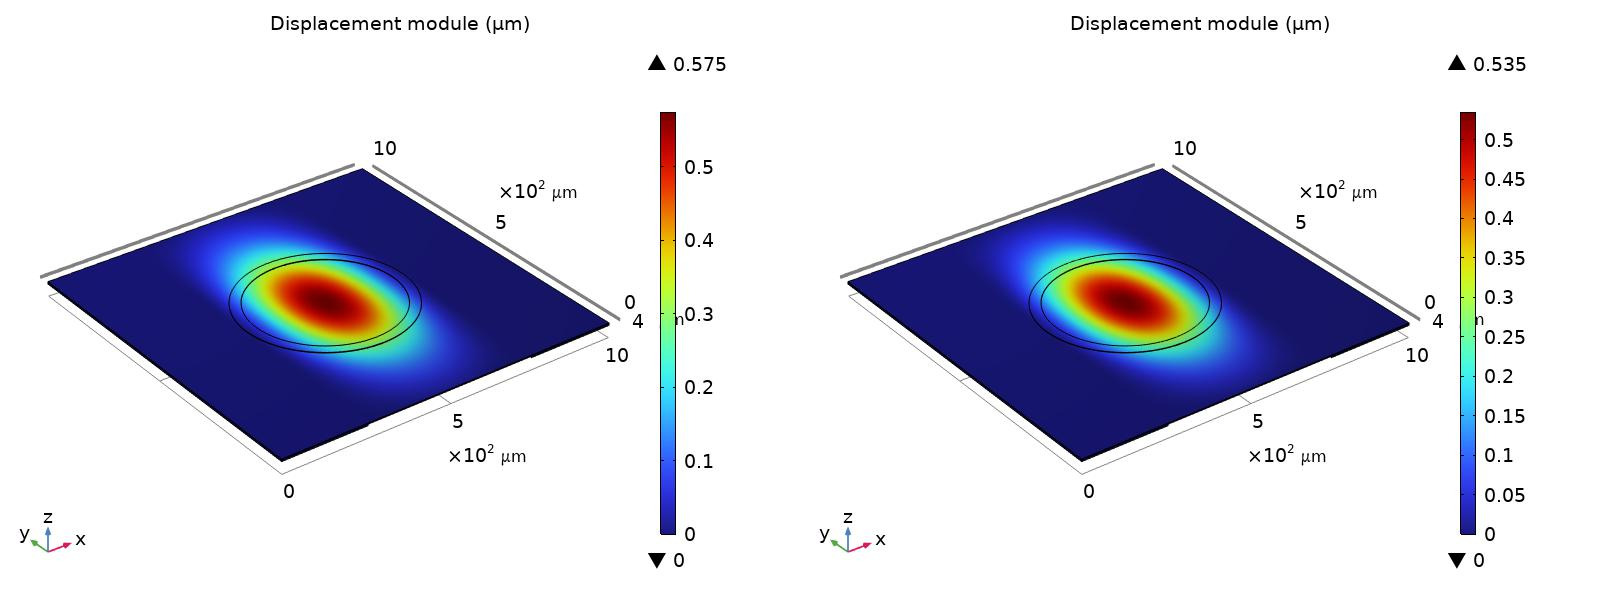
\includegraphics[width=1\linewidth]{img/displacement_mesh_impact_perf_back.jpg}
    \caption{Mesh impact on displacement for perforated back structure: \\
    left is normal quality mesh, right is extra-coarse quality mesh}
    \label{fig:displacement_mesh_impact_perf_back}
\end{figure}

\begin{figure}[h!]
    \centering
    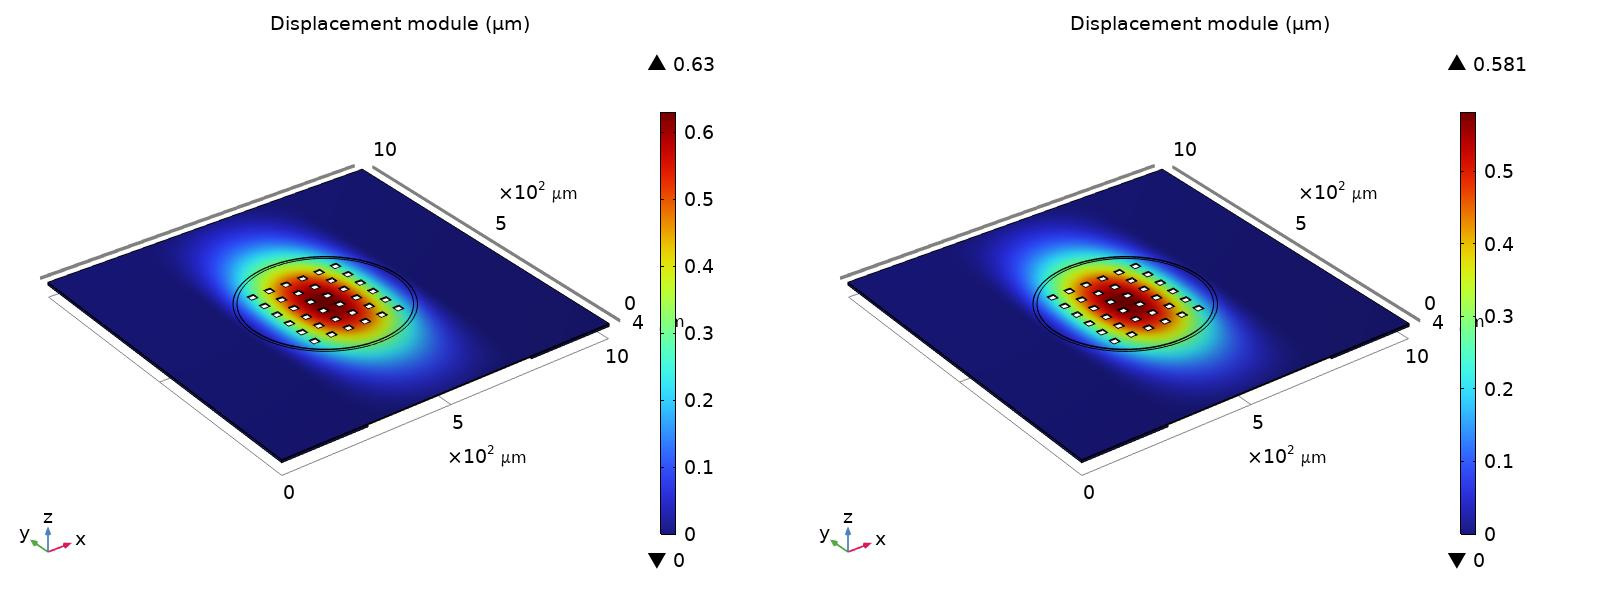
\includegraphics[width=1\linewidth]{img/displacement_mesh_impact_perf_diaph.jpg}
    \caption{Mesh impact on displacement for perforated diaphragm structure: \\
    left is normal quality mesh, right is extra-coarse quality mesh}
    \label{fig:displacement_mesh_impact_perf_diaph}
\end{figure}

\noindent
As we can see from \autoref{fig:displacement_mesh_impact_perf_back} and \autoref{fig:displacement_mesh_impact_perf_diaph}, the maximum displacement values decrease for both types of structure as the mesh quality decreases; this means that the larger displacement value shown is a more accurate approximation of the real value. \\
Obviously, these results are different from the ones obtained before, because the structures analyzed are simpler (to allow the computation with a higher-quality mesh). \\
These simulations has been done considering a diaphragm thickness (\texttt{t\_d}) of \(3 \; \mu m\), an applied voltage (\texttt{V\_x}) of \(0 \; V\) and an external pressure applied (\texttt{P\_x}) of \(1000 \; Pa\).
It can be interesting to evaluate the relative error induced by the mesh quality.
To calculate this, the formula \cref{eq:epsilon_r_formula} has been used.

\begin{equation}
    \varepsilon_r = \frac{ \left. f( \vec{r}) \right|_{\text{normal mesh}} - \left. f( \vec{r}) \right|_{\text{extra-coarse mesh}}}{\left. f( \vec{r}) \right|_{\text{normal mesh}}}
    \label{eq:epsilon_r_formula}
\end{equation}

\noindent
The absolute value of displacement relative errors are given by \cref{eq:epsilon_r_disp_perf_back} for the perforated back structure and by \cref{eq:epsilon_r_disp_perf_diap} for the perforated diaphragm structure.

\begin{equation}
    \left| \varepsilon_r \right|_{\text{perf. back}} \simeq \frac{0.575 \; \mu m - 0.535 \; \mu m}{0.575 \; \mu m} \simeq 0.0696
    \label{eq:epsilon_r_disp_perf_back}
\end{equation}

\begin{equation}
    \left| \varepsilon_r \right|_{\text{perf. diap.}} \simeq \frac{0.635 \; \mu m - 0.581 \; \mu m}{0.635 \; \mu m} \simeq 0.085
    \label{eq:epsilon_r_disp_perf_diap}
\end{equation}

\begin{figure}[h!]
    \centering
    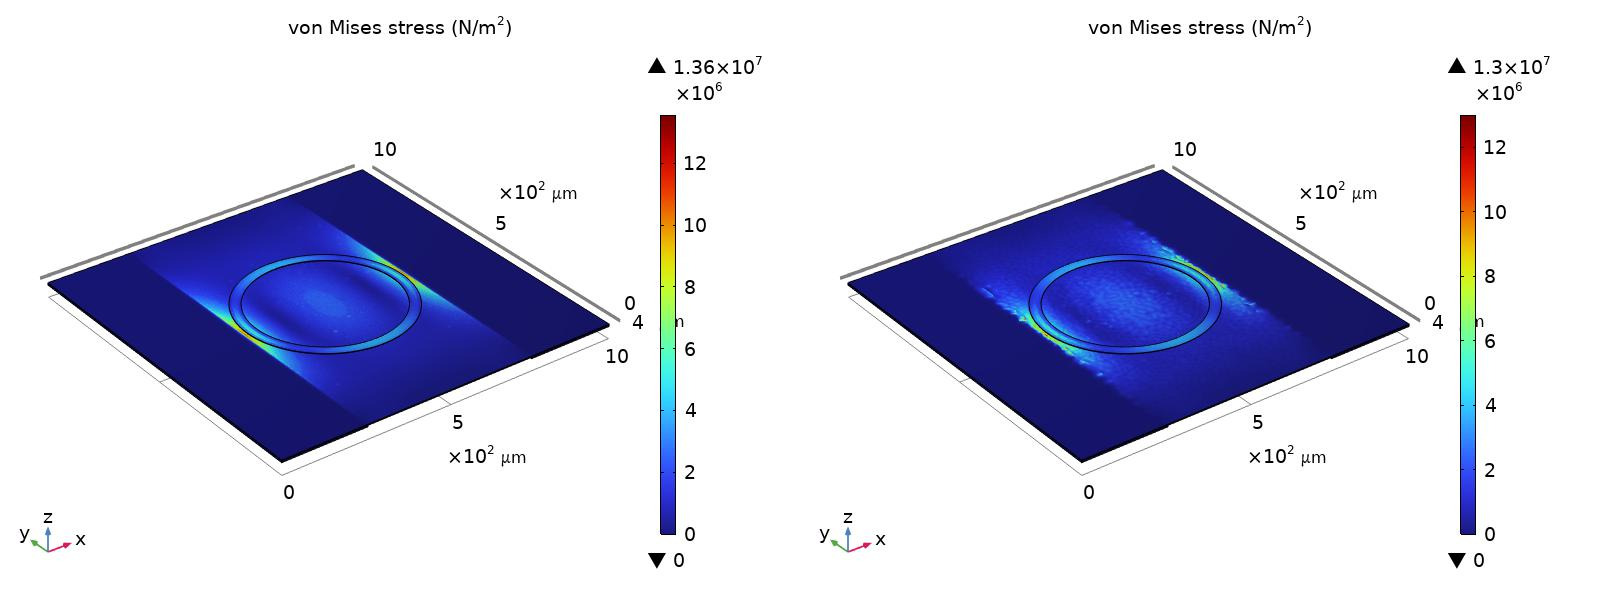
\includegraphics[width=1\linewidth]{img/stress_mesh_impact_perf_back.jpg}
    \caption{Mesh impact on von Mises stress for perforated back structure: \\
    left is normal quality mesh, right is extra-coarse quality mesh}
    \label{fig:stress_mesh_impact_perf_back}
\end{figure}

\begin{figure}[h!]
    \centering
    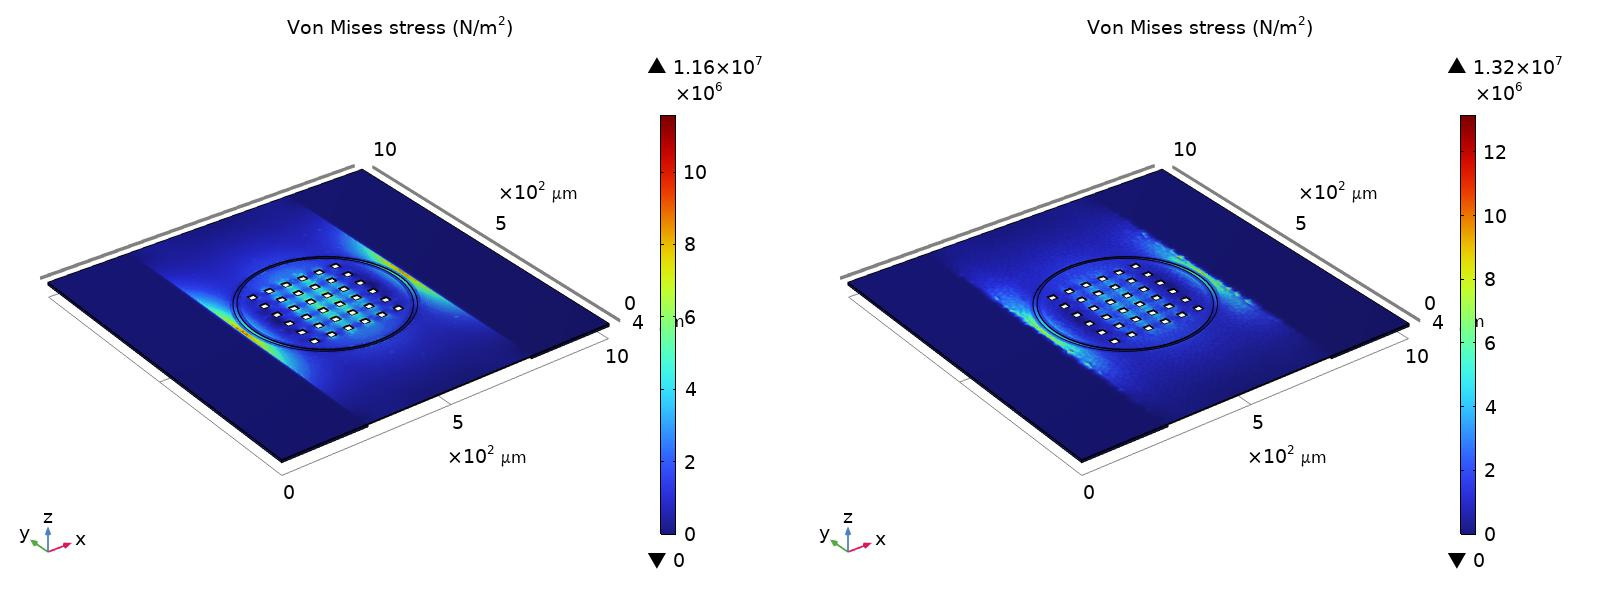
\includegraphics[width=1\linewidth]{img/stress_mesh_impact_perf_diaph.jpg}
    \caption{Mesh impact on von Mises stress for perforated diaphragm structure: \\
    left is normal quality mesh, right is extra-coarse quality mesh}
    \label{fig:stress_mesh_impact_perf_diaph}
\end{figure}

\noindent
The same evaluations has been done for the von Mises stress values as shown in \autoref{fig:stress_mesh_impact_perf_back} and \autoref{fig:stress_mesh_impact_perf_diaph}. \\
Differently from before, this time the evaluated maximum stress value does not decrease for both types of structure with the mesh quality. \\
This behavior can be caused by the peak value near the lateral border; probably, for a correct evaluation of that value, the mesh in that region must be very fine, otherwise the value is poorly approximated. \\
These simulations have been done with the same parameters as before, and by using the same formula to evaluate the absolute value of relative error (\cref{eq:epsilon_r_formula}), we can extract the errors for the stress values, which are respectively given by \cref{eq:epsilon_r_stress_perf_back} for the perforated back structure and \cref{eq:epsilon_r_stress_perf_diap} for the perforated diaphragm structure.

\begin{equation}
    \left| \varepsilon_r \right|_{\text{perf. back}} \simeq \frac{13.6 \; \frac{N}{mm^2} - 13 \; \frac{N}{mm^2}}{13.6 \; \frac{N}{mm^2}} \simeq 0.0441
    \label{eq:epsilon_r_stress_perf_back}
\end{equation}

\begin{equation}
    \left| \varepsilon_r \right|_{\text{perf. diap.}} \simeq \frac{13.2 \; \frac{N}{mm^2} - 11.6 \; \frac{N}{mm^2}}{11.6 \; \frac{N}{mm^2}} \simeq 0.138
    \label{eq:epsilon_r_stress_perf_diap}
\end{equation}

\noindent
As we can see from these results, the error goes from an approximately \(8.5 \%\) value for the displacement up to approximately \(13.8 \%\) for the stress values. \\
These error values are significant and may have caused the main difference from the results in the reference paper \cite{krishnapriya2014}.

\subsection{Comparison with analytical model and physical devices}

The last comparison done is the validity of the approximated analytical formula (found in the following paper \cite[p.~988-989]{jerman1986} for shallow, sinusoidal corrugated diaphragm) for the deflection of the membrane \cref{eq:diaphragm_deflection}. \\
To compute that, the following formula \cref{eq:plotted_disp_equation} has been plotted.

\begin{equation}
     \begin{cases}
        P = \frac{a_p}{\theta} \frac{y}{h} + \frac{b_p}{\theta} \frac{y^3}{h^3} \\
        \\
        \theta = \frac{R^4}{E'h^4}
    \end{cases}
    \label{eq:plotted_disp_equation}
\end{equation}

\noindent
The resulting graph has the pressure along the y-axis and the maximum displacement on the x-axis. \\
The displacement value associated with a specific pressure corresponds to the intersection of the graph with the function \(P=\texttt{P\_x}\), which corresponds to a horizontal line on the graph.
The data used for simulation, and to plot the graph are:

\begin{itemize}
    \item \textbf{h}: \(3 \; \mu m\) diaphragm thickness
    \item \textbf{H}: \(0,5 \cdot \text{h} = 1.5 \; \mu m\) corrugation depth
    \item \textbf{E}: \(70 \cdot 10^9 \; Pa\) Young's modulus for aluminum
    \item \textbf{v}: \(0.35\) Poisson's ratio for aluminum
    \item \textbf{R}: \(210 \; \mu m\) membrane ratio
\end{itemize}

\noindent
The resulting graph with the following values is shown in \autoref{fig:pressure_vs_disp}.

\begin{figure}[h!]
    \centering
    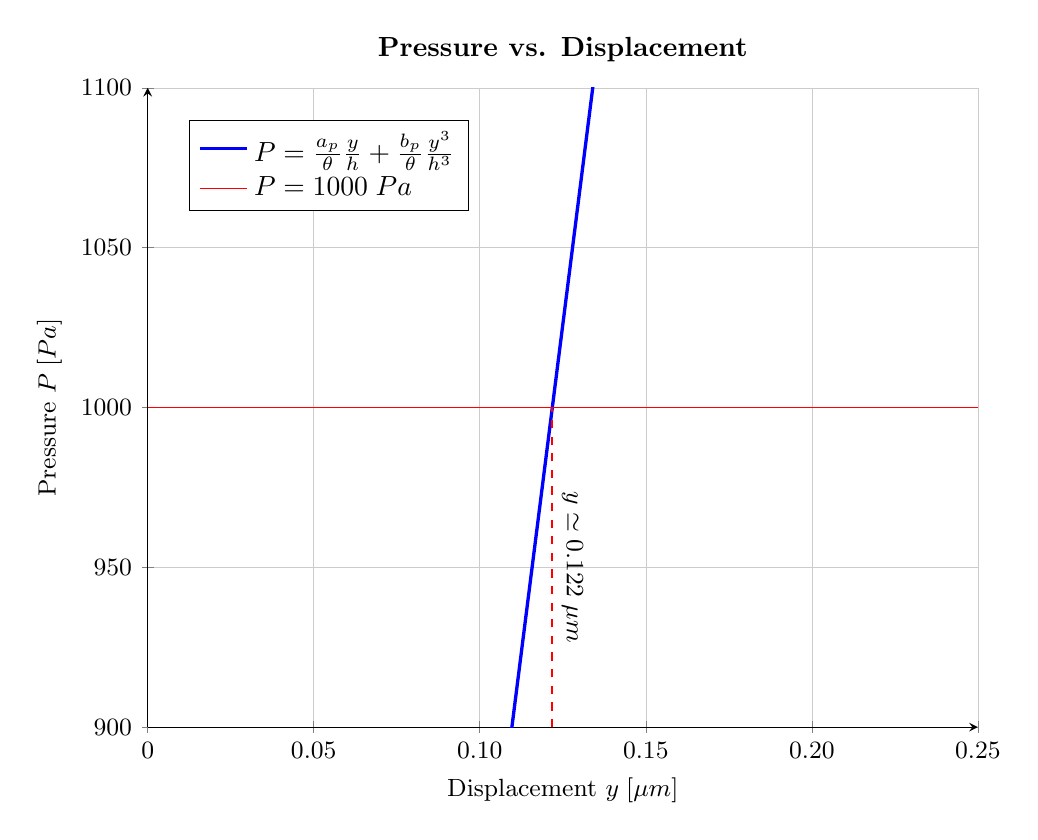
\begin{tikzpicture}
        \begin{axis}[
            width=\columnwidth,
            height=0.8\columnwidth,
            axis lines=left,
            xlabel={Displacement $y\;[\mu m]$},
            ylabel={Pressure $P\;[Pa]$},
            xmin=0, xmax=0.25,
            ymin=900, ymax=1100,
            grid=both,
            grid style={line width=.1pt, draw=gray!20},
            major grid style={line width=.2pt,draw=gray!40},
            legend style={at={(0.05,0.95)},anchor=north west},
            title={Pressure vs. Displacement},
            xtick = {0, 0.05, 0.1, 0.15, 0.2, 0.25},
            xticklabels = {$0$, $0.05$, $0.10$, $0.15$, $0.20$, $0.25$},
            ytick = {900, 950, 1000, 1050, 1100},
            yticklabels = {$900$, $950$, $1000$, $1050$, $1100$},
            title style={font=\bfseries},
            tick label style={font=\small},
            label style={font=\small},
            legend cell align={left}
        ]
        
        % Curve
        \addplot [blue, very thick, domain=0:0.25] {24609*x/3 + 7466*(x/3)^3};
        \addlegendentry{$P = \frac{a_p}{\theta} \frac{y}{h} + \frac{b_p}{\theta} \frac{y^3}{h^3}$}
        
        % Horizontal line
        \addplot [red, very thin] coordinates {(0,1000) (0.25,1000)};
        \addlegendentry{$P = 1000 \; Pa$}
    
        % Vertical line
        \addplot [red, dashed, thick] coordinates {(0.12184,900) (0.12184,1000)};
        \node[rotate=270, anchor=south, font=\small] at (axis cs:0.12184,950) {$y \simeq 0.122 \; \mu m$};
        
        \end{axis}

    \end{tikzpicture}

    \caption{Analytical pressure function plotted as a function of displacement}
    \label{fig:pressure_vs_disp}

\end{figure}

\noindent
As we can see from \autoref{fig:pressure_vs_disp}, the maximum displacement value at a pressure of \(1000 \; Pa\) is \(0.122 \; \mu m\), which is significantly different from the simulated results and from the values reported in the paper. \\
This confirms that the analytical function is only useful to get an idea of the order of magnitude we are working with.

\subsection{Final conclusions}

The simulations performed produced different results, and many parameters have been neglected. \\
The results vary significantly depending on several factors: mesh quality, model accuracy (simulating the entire device is different from simulating only the diaphragm), the analytical equations and the physical modules used for the simulations, etc. \\
For this reason, the mathematical approximated model and the simulations should only be used to size the structure, allowing us to understand the order of magnitude we are dealing with. \\
However, to design a proper MEMS microphone structure, many physical tests are required, because for complex structures like the one considered here, the results can differ significantly from the real ones. \\
Naturally, \textbf{COMSOL 6.4} is a powerful simulation tool that allows the coupling of different modules; the more physical modules are used, the more accurate the simulation results are, but the more complex the model becomes. \\
At a certain level of complexity, it becomes more convenient to perform simplified simulations and rely on physical tests.
